\documentclass[12pt,twoside]{article}

\usepackage{amsmath}
\usepackage{color}
\usepackage{enumitem}
\usepackage{graphicx}
\graphicspath{ {images/} }

\usepackage{subfig}
\usepackage{placeins}
\usepackage{float}

\usepackage{mdframed}

\newcommand{\head}[1]{\textnormal{\textbf{#1}}}

\newcommand{\cross}[1][1pt]{\ooalign{%
  \rule[1ex]{1ex}{#1}\cr% Horizontal bar
  \hss\rule{#1}{.7em}\hss\cr}}% Vertical bar

% Cross-references for handout numbers.

\newcommand{\name}{}

\usepackage{latexsym}
%\usepackage{bbm}
\usepackage{times,url}
\usepackage{clrscode}

\newcommand{\mitst}[1]{\begin{description}
\item[MIT students:] #1
\end{description}}
\newcommand{\smast}[1]{\begin{description}
\item[SMA students:] #1
\end{description}}

\newcommand{\profs}{Professor Chris Rycroft}
\newcommand{\subj}{AM205}

\newlength{\toppush}
\setlength{\toppush}{2\headheight}
\addtolength{\toppush}{\headsep}

\newcommand{\htitle}[2]{\noindent\vspace*{-\toppush}\newline\parbox{6.5in}
{\textit{Advanced Scientific Computing: Numerical Methods AM205}\hfill\name\newline
Harvard University \hfill #2\newline
\profs\hfill #1 \vspace*{-.5ex}\newline
\mbox{}\hrulefill\mbox{}}\vspace*{1ex}\mbox{}\newline
\begin{center}{\Large\bf #1}\end{center}}

\newcommand{\handout}[2]{\thispagestyle{empty}
 \markboth{#1}{#1}
 \pagestyle{myheadings}\htitle{#1}{#2}}

\newcommand{\htitlewithouttitle}[2]{\noindent\vspace*{-\toppush}\newline\parbox{6.5in}
{\textit{Introduction to Algorithms}\hfill#2\newline
Massachusetts Institute of Technology \hfill 6.006\newline
%Singapore-MIT Alliance \hfill SMA5503\newline
\profs\hfill Handout #1\vspace*{-.5ex}\newline
\mbox{}\hrulefill\mbox{}}\vspace*{1ex}\mbox{}\newline}

\newcommand{\handoutwithouttitle}[2]{\thispagestyle{empty}
 \markboth{Handout \protect\ref{#1}}{Handout \protect\ref{#1}}
 \pagestyle{myheadings}\htitlewithouttitle{\protect\ref{#1}}{#2}}

\newcommand{\exam}[2]{% parameters: exam name, date
 \thispagestyle{empty}
 \markboth{\subj\ #1\hspace{1in}Name\hrulefill\ \ }%
          {\subj\ #1\hspace{1in}Name\hrulefill\ \ }
 \pagestyle{myheadings}\examtitle{#1}{#2}
 \renewcommand{\theproblem}{Problem \arabic{problemnum}}
}
\newcommand{\examsolutions}[3]{% parameters: handout, exam name, date
 \thispagestyle{empty}
 \markboth{Handout \protect\ref{#1}: #2}{Handout \protect\ref{#1}: #2}
% \pagestyle{myheadings}\htitle{\protect\ref{#1}}{#2}{#3}
 \pagestyle{myheadings}\examsolutionstitle{\protect\ref{#1}} {#2}{#3}
 \renewcommand{\theproblem}{Problem \arabic{problemnum}}
}
\newcommand{\examsolutionstitle}[3]{\noindent\vspace*{-\toppush}\newline\parbox{6.5in}
{\textit{Introduction to Algorithms}\hfill#3\newline
Massachusetts Institute of Technology \hfill 6.006\newline
%Singapore-MIT Alliance \hfill SMA5503\newline
\profs\hfill Handout #1\vspace*{-.5ex}\newline
\mbox{}\hrulefill\mbox{}}\vspace*{1ex}\mbox{}\newline
\begin{center}{\Large\bf #2}\end{center}}

\newcommand{\takehomeexam}[2]{% parameters: exam name, date
 \thispagestyle{empty}
 \markboth{\subj\ #1\hfill}{\subj\ #1\hfill}
 \pagestyle{myheadings}\examtitle{#1}{#2}
 \renewcommand{\theproblem}{Problem \arabic{problemnum}}
}

\makeatletter
\newcommand{\exambooklet}[2]{% parameters: exam name, date
 \thispagestyle{empty}
 \markboth{\subj\ #1}{\subj\ #1}
 \pagestyle{myheadings}\examtitle{#1}{#2}
 \renewcommand{\theproblem}{Problem \arabic{problemnum}}
 \renewcommand{\problem}{\newpage
 \item \let\@currentlabel=\theproblem
 \markboth{\subj\ #1, \theproblem}{\subj\ #1, \theproblem}}
}
\makeatother


\newcommand{\examtitle}[2]{\noindent\vspace*{-\toppush}\newline\parbox{6.5in}
{\textit{Advanced Scientific Computing: Numerical Methods}\hfill#2\newline
Harvard University \hfill AM205 Fall 2017\newline
%Singapore-MIT Alliance \hfill SMA5503\newline
\profs\hfill #1\vspace*{-.5ex}\newline
\mbox{}\hrulefill\mbox{}}\vspace*{1ex}\mbox{}\newline
\begin{center}{\Large\bf #1}\end{center}}

\newcommand{\grader}[1]{\hspace{1cm}\textsf{\textbf{#1}}\hspace{1cm}}

\newcommand{\points}[1]{[#1 points]\ }
\newcommand{\parts}[1]
{
  \ifnum#1=1
  (1 part)
  \else
  (#1 parts)
  \fi
  \
}

\newcommand{\bparts}{\begin{problemparts}}
\newcommand{\eparts}{\end{problemparts}}
\newcommand{\ppart}{\problempart}

%\newcommand{\lg} {lg\ }

\setlength{\oddsidemargin}{0pt}
\setlength{\evensidemargin}{0pt}
\setlength{\textwidth}{6.5in}
\setlength{\topmargin}{0in}
\setlength{\textheight}{8.5in}


\newcommand{\Spawn}{{\bf spawn} }
\newcommand{\Sync}{{\bf sync}}

\renewcommand{\cases}[1]{\left\{ \begin{array}{ll}#1\end{array}\right.}
\newcommand{\cif}[1]{\mbox{if $#1$}}
\newcommand{\cwhen}[1]{\mbox{when $#1$}}

\newcounter{problemnum}
\newcommand{\theproblem}{Problem \theproblemsetnum-\arabic{problemnum}}
\newenvironment{problems}{
        \begin{list}{{\bf \theproblem. \hspace*{0.5em}}}
        {\setlength{\leftmargin}{0em}
         \setlength{\rightmargin}{0em}
         \setlength{\labelwidth}{0em}
         \setlength{\labelsep}{0em}
         \usecounter{problemnum}}}{\end{list}}
\makeatletter
\newcommand{\problem}[1][{}]{\item \let\@currentlabel=\theproblem \textbf{#1}}
\makeatother

\newcounter{problempartnum}[problemnum]
\newenvironment{problemparts}{
        \begin{list}{{\bf (\alph{problempartnum})}}
        {\setlength{\leftmargin}{2.5em}
         \setlength{\rightmargin}{2.5em}
         \setlength{\labelsep}{0.5em}}}{\end{list}}
\newcommand{\problempart}{\addtocounter{problempartnum}{1}\item}

\newenvironment{truefalseproblemparts}{
        \begin{list}{{\bf (\alph{problempartnum})\ \ \ T\ \ F\hfil}}
        {\setlength{\leftmargin}{4.5em}
         \setlength{\rightmargin}{2.5em}
         \setlength{\labelsep}{0.5em}
         \setlength{\labelwidth}{4.5em}}}{\end{list}}

\newcounter{exercisenum}
\newcommand{\theexercise}{Exercise \theproblemsetnum-\arabic{exercisenum}}
\newenvironment{exercises}{
        \begin{list}{{\bf \theexercise. \hspace*{0.5em}}}
        {\setlength{\leftmargin}{0em}
         \setlength{\rightmargin}{0em}
         \setlength{\labelwidth}{0em}
         \setlength{\labelsep}{0em}
        \usecounter{exercisenum}}}{\end{list}}
\makeatletter
\newcommand{\exercise}{\item \let\@currentlabel=\theexercise}
\makeatother

\newcounter{exercisepartnum}[exercisenum]
%\newcommand{\problem}[1]{\medskip\mbox{}\newline\noindent{\bf Problem #1.}\hspace*{1em}}
%\newcommand{\exercise}[1]{\medskip\mbox{}\newline\noindent{\bf Exercise #1.}\hspace*{1em}}

\newenvironment{exerciseparts}{
        \begin{list}{{\bf (\alph{exercisepartnum})}}
        {\setlength{\leftmargin}{2.5em}
         \setlength{\rightmargin}{2.5em}
         \setlength{\labelsep}{0.5em}}}{\end{list}}
\newcommand{\exercisepart}{\addtocounter{exercisepartnum}{1}\item}


% Macros to make captions print with small type and 'Figure xx' in bold.
\makeatletter
\def\fnum@figure{{\bf Figure \thefigure}}
\def\fnum@table{{\bf Table \thetable}}
\let\@mycaption\caption
%\long\def\@mycaption#1[#2]#3{\addcontentsline{\csname
%  ext@#1\endcsname}{#1}{\protect\numberline{\csname
%  the#1\endcsname}{\ignorespaces #2}}\par
%  \begingroup
%    \@parboxrestore
%    \small
%    \@makecaption{\csname fnum@#1\endcsname}{\ignorespaces #3}\par
%  \endgroup}
%\def\mycaption{\refstepcounter\@captype \@dblarg{\@mycaption\@captype}}
%\makeatother
\let\mycaption\caption
%\newcommand{\figcaption}[1]{\mycaption[]{#1}}

\newcounter{totalcaptions}
\newcounter{totalart}

\newcommand{\figcaption}[1]{\addtocounter{totalcaptions}{1}\caption[]{#1}}

% \psfigures determines what to do for figures:
%       0 means just leave vertical space
%       1 means put a vertical rule and the figure name
%       2 means insert the PostScript version of the figure
%       3 means put the figure name flush left or right
\newcommand{\psfigures}{0}
\newcommand{\spacefigures}{\renewcommand{\psfigures}{0}}
\newcommand{\rulefigures}{\renewcommand{\psfigures}{1}}
\newcommand{\macfigures}{\renewcommand{\psfigures}{2}}
\newcommand{\namefigures}{\renewcommand{\psfigures}{3}}

\newcommand{\figpart}[1]{{\bf (#1)}\nolinebreak[2]\relax}
\newcommand{\figparts}[2]{{\bf (#1)--(#2)}\nolinebreak[2]\relax}


\macfigures     % STATE

% When calling \figspace, make sure to leave a blank line afterward!!
% \widefigspace is for figures that are more than 28pc wide.
\newlength{\halffigspace} \newlength{\wholefigspace}
\newlength{\figruleheight} \newlength{\figgap}
\newcommand{\setfiglengths}{\ifnum\psfigures=1\setlength{\figruleheight}{\hruleheight}\setlength{\figgap}{1em}\else\setlength{\figruleheight}{0pt}\setlength{\figgap}{0em}\fi}
\newcommand{\figspace}[2]{\ifnum\psfigures=0\leavefigspace{#1}\else%
\setfiglengths%
\setlength{\wholefigspace}{#1}\setlength{\halffigspace}{.5\wholefigspace}%
\rule[-\halffigspace]{\figruleheight}{\wholefigspace}\hspace{\figgap}#2\fi}
\newlength{\widefigspacewidth}
% Make \widefigspace put the figure flush right on the text page.
\newcommand{\widefigspace}[2]{
\ifnum\psfigures=0\leavefigspace{#1}\else%
\setfiglengths%
\setlength{\widefigspacewidth}{28pc}%
\addtolength{\widefigspacewidth}{-\figruleheight}%
\setlength{\wholefigspace}{#1}\setlength{\halffigspace}{.5\wholefigspace}%
\makebox[\widefigspacewidth][r]{#2\hspace{\figgap}}\rule[-\halffigspace]{\figruleheight}{\wholefigspace}\fi}
\newcommand{\leavefigspace}[1]{\setlength{\wholefigspace}{#1}\setlength{\halffigspace}{.5\wholefigspace}\rule[-\halffigspace]{0em}{\wholefigspace}}

% Commands for including figures with macpsfig.
% To use these commands, documentstyle ``macpsfig'' must be specified.
\newlength{\macfigfill}
\makeatother
\newlength{\bbx}
\newlength{\bby}
\newcommand{\macfigure}[5]{\addtocounter{totalart}{1}
\ifnum\psfigures=2%
\setlength{\bbx}{#2}\addtolength{\bbx}{#4}%
\setlength{\bby}{#3}\addtolength{\bby}{#5}%
\begin{flushleft}
\ifdim#4>28pc\setlength{\macfigfill}{#4}\addtolength{\macfigfill}{-28pc}\hspace*{-\macfigfill}\fi%
\mbox{\psfig{figure=./#1.ps,%
bbllx=#2,bblly=#3,bburx=\bbx,bbury=\bby}}
\end{flushleft}%
\else\ifdim#4>28pc\widefigspace{#5}{#1}\else\figspace{#5}{#1}\fi\fi}
\makeatletter

\newlength{\savearraycolsep}
\newcommand{\narrowarray}[1]{\setlength{\savearraycolsep}{\arraycolsep}\setlength{\arraycolsep}{#1\arraycolsep}}
\newcommand{\normalarray}{\setlength{\arraycolsep}{\savearraycolsep}}

\newcommand{\hint}{{\em Hint:\ }}

% Macros from /th/u/clr/mac.tex

\newcommand{\set}[1]{\left\{ #1 \right\}}
\newcommand{\abs}[1]{\left| #1\right|}
\newcommand{\card}[1]{\left| #1\right|}
\newcommand{\floor}[1]{\left\lfloor #1 \right\rfloor}
\newcommand{\ceil}[1]{\left\lceil #1 \right\rceil}
\newcommand{\ang}[1]{\ifmmode{\left\langle #1 \right\rangle}
   \else{$\left\langle${#1}$\right\rangle$}\fi}
        % the \if allows use outside mathmode,
        % but will swallow following space there!
\newcommand{\paren}[1]{\left( #1 \right)}
\newcommand{\bracket}[1]{\left[ #1 \right]}
\newcommand{\prob}[1]{\Pr\left\{ #1 \right\}}
\newcommand{\Var}{\mathop{\rm Var}\nolimits}
\newcommand{\expect}[1]{{\rm E}\left[ #1 \right]}
\newcommand{\expectsq}[1]{{\rm E}^2\left[ #1 \right]}
\newcommand{\variance}[1]{{\rm Var}\left[ #1 \right]}
\renewcommand{\choose}[2]{{{#1}\atopwithdelims(){#2}}}
\def\pmod#1{\allowbreak\mkern12mu({\rm mod}\,\,#1)}
\newcommand{\matx}[2]{\left(\begin{array}{*{#1}{c}}#2\end{array}\right)}
\newcommand{\Adj}{\mathop{\rm Adj}\nolimits}

\newtheorem{theorem}{Theorem}
\newtheorem{lemma}[theorem]{Lemma}
\newtheorem{corollary}[theorem]{Corollary}
\newtheorem{xample}{Example}
\newtheorem{definition}{Definition}
\newenvironment{example}{\begin{xample}\rm}{\end{xample}}
\newcommand{\proof}{\noindent{\em Proof.}\hspace{1em}}
\def\squarebox#1{\hbox to #1{\hfill\vbox to #1{\vfill}}}
\newcommand{\qedbox}{\vbox{\hrule\hbox{\vrule\squarebox{.667em}\vrule}\hrule}}
\newcommand{\qed}{\nopagebreak\mbox{}\hfill\qedbox\smallskip}
\newcommand{\eqnref}[1]{(\protect\ref{#1})}

%%\newcommand{\twodots}{\mathinner{\ldotp\ldotp}}
\newcommand{\transpose}{^{\mbox{\scriptsize \sf T}}}
\newcommand{\amortized}[1]{\widehat{#1}}

\newcommand{\punt}[1]{}

%%% command for putting definitions into boldface
% New style for defined terms, as of 2/23/88, redefined by THC.
\newcommand{\defn}[1]{{\boldmath\textit{\textbf{#1}}}}
\newcommand{\defi}[1]{{\textit{\textbf{#1\/}}}}

\newcommand{\red}{\leq_{\rm P}}
\newcommand{\lang}[1]{%
\ifmmode\mathord{\mathcode`-="702D\rm#1\mathcode`\-="2200}\else{\rm#1}\fi}

%\newcommand{\ckt}[1]{\ifmmode\mathord{\mathcode`-="702D\sc #1\mathcode`\-="2200}\else$\mathord{\mathcode`-="702D\sc #1\mathcode`\-="2200}$\fi}
\newcommand{\ckt}[1]{\ifmmode \sc #1\else$\sc #1$\fi}

%% Margin notes - use \notesfalse to turn off notes.
\setlength{\marginparwidth}{0.6in}
\reversemarginpar
\newif\ifnotes
\notestrue
\newcommand{\longnote}[1]{
  \ifnotes
    {\medskip\noindent Note: \marginpar[\hfill$\Longrightarrow$]
      {$\Longleftarrow$}{#1}\medskip}
  \fi}
\newcommand{\note}[1]{
  \ifnotes
    {\marginpar{\tiny \raggedright{#1}}}
  \fi}


\newcommand{\reals}{\mathbbm{R}}
\newcommand{\integers}{\mathbbm{Z}}
\newcommand{\naturals}{\mathbbm{N}}
\newcommand{\rationals}{\mathbbm{Q}}
\newcommand{\complex}{\mathbbm{C}}

\newcommand{\oldreals}{{\bf R}}
\newcommand{\oldintegers}{{\bf Z}}
\newcommand{\oldnaturals}{{\bf N}}
\newcommand{\oldrationals}{{\bf Q}}
\newcommand{\oldcomplex}{{\bf C}}

\newcommand{\w}{\omega}                 %% for fft chapter

\newenvironment{closeitemize}{\begin{list}
{$\bullet$}
{\setlength{\itemsep}{-0.2\baselineskip}
\setlength{\topsep}{0.2\baselineskip}
\setlength{\parskip}{0pt}}}
{\end{list}}

% These are necessary within a {problems} environment in order to restore
% the default separation between bullets and items.
\newenvironment{normalitemize}{\setlength{\labelsep}{0.5em}\begin{itemize}}
                              {\end{itemize}}
\newenvironment{normalenumerate}{\setlength{\labelsep}{0.5em}\begin{enumerate}}
                                {\end{enumerate}}

%\def\eqref#1{Equation~(\ref{eq:#1})}
%\newcommand{\eqref}[1]{Equation (\ref{eq:#1})}
\newcommand{\eqreftwo}[2]{Equations (\ref{eq:#1}) and~(\ref{eq:#2})}
\newcommand{\ineqref}[1]{Inequality~(\ref{ineq:#1})}
\newcommand{\ineqreftwo}[2]{Inequalities (\ref{ineq:#1}) and~(\ref{ineq:#2})}

\newcommand{\figref}[1]{Figure~\ref{fig:#1}}
\newcommand{\figreftwo}[2]{Figures \ref{fig:#1} and~\ref{fig:#2}}

\newcommand{\liref}[1]{line~\ref{li:#1}}
\newcommand{\Liref}[1]{Line~\ref{li:#1}}
\newcommand{\lirefs}[2]{lines \ref{li:#1}--\ref{li:#2}}
\newcommand{\Lirefs}[2]{Lines \ref{li:#1}--\ref{li:#2}}
\newcommand{\lireftwo}[2]{lines \ref{li:#1} and~\ref{li:#2}}
\newcommand{\lirefthree}[3]{lines \ref{li:#1}, \ref{li:#2}, and~\ref{li:#3}}

\newcommand{\lemlabel}[1]{\label{lem:#1}}
\newcommand{\lemref}[1]{Lemma~\ref{lem:#1}}

\newcommand{\exref}[1]{Exercise~\ref{ex:#1}}

\newcommand{\handref}[1]{Handout~\ref{#1}}

\newcommand{\defref}[1]{Definition~\ref{def:#1}}

% (1997.8.16: Victor Luchangco)
% Modified \hlabel to only get date and to use handouts counter for number.
%   New \handout and \handoutwithouttitle commands in newmac.tex use this.
%   The date is referenced by <label>-date.
%   (Retained old definition as \hlabelold.)
%   Defined \hforcelabel to use an argument instead of the handouts counter.

\newcounter{handouts}
\setcounter{handouts}{0}

\newcommand{\hlabel}[2]{%
\stepcounter{handouts}
{\edef\next{\write\@auxout{\string\newlabel{#1}{{\arabic{handouts}}{0}}}}\next}
\write\@auxout{\string\newlabel{#1-date}{{#2}{0}}}
}

\newcommand{\hforcelabel}[3]{%          Does not step handouts counter.
\write\@auxout{\string\newlabel{#1}{{#2}{0}}}
\write\@auxout{\string\newlabel{#1-date}{{#3}{0}}}}


% less ugly underscore
% --juang, 2008 oct 05
\renewcommand{\_}{\vrule height 0 pt depth 0.4 pt width 0.5 em \,}


\setlength{\oddsidemargin}{0pt}
\setlength{\evensidemargin}{0pt}
\setlength{\textwidth}{6.5in}
\setlength{\topmargin}{0in}
\setlength{\textheight}{8.5in}

\newcommand{\theproblemsetnum}{}
\newcommand{\releasedate}{December 1, 2017}
\newcommand{\duedate}{December 1, 2017}
\newcommand{\tabUnit}{3ex}
\newcommand{\tabT}{\hspace*{\tabUnit}}

\usepackage{listings}
\usepackage{color}
\usepackage{amsmath}


\definecolor{dkgreen}{rgb}{0,0.6,0}
\definecolor{gray}{rgb}{0.5,0.5,0.5}
\definecolor{mauve}{rgb}{0.58,0,0.82}

\lstset{frame=tb,
  language=Python,
  aboveskip=3mm,
  belowskip=3mm,
  showstringspaces=false,
  columns=flexible,
  basicstyle={\small\ttfamily},
  numbers=none,
  numberstyle=\tiny\color{gray},
  keywordstyle=\color{blue},
  commentstyle=\color{dkgreen},
  stringstyle=\color{mauve},
  breaklines=true,
  breakatwhitespace=true,
  tabsize=3
}

\title{6.006 Problem Set 4}

\begin{document}

\handout{Crypto project \theproblemsetnum}{\releasedate} %{April 6, 2017}

\setlength{\parindent}{0pt}

\medskip

\hrulefill

\medskip

{\bf Name:} Yihang Yan, Tomas Gudmundsson, Nathaniel Stein

\medskip

{\bf Collaborators:} None

\medskip

\hrulefill

%%%%%%%%%%%%%%%%%%%%%%%%%%%%%%%%%%%%%%%%%%%%%%%%%%%%%
% See below for common and useful latex constructs. %
%%%%%%%%%%%%%%%%%%%%%%%%%%%%%%%%%%%%%%%%%%%%%%%%%%%%%

% Some useful commands:
%$f(x) = \Theta(x)$
%$T(x, y) \leq \log(x) + 2^y + \binom{2n}{n}$
% {\tt code\_function}


% You can create unnumbered lists as follows:
%\begin{itemize}
%    \item First item in a list 
%        \begin{itemize}
%            \item First item in a list 
%                \begin{itemize}
%                    \item First item in a list 
%                    \item Second item in a list 
%                \end{itemize}
%            \item Second item in a list 
%        \end{itemize}
%    \item Second item in a list 
%\end{itemize}

% You can create numbered lists as follows:
%\begin{enumerate}
%    \item First item in a list 
%    \item Second item in a list 
%    \item Third item in a list
%\end{enumerate}

% You can write aligned equations as follows:
%\begin{align} 
%    \begin{split}
%        (x+y)^3 &= (x+y)^2(x+y) \\
%                &= (x^2+2xy+y^2)(x+y) \\
%                &= (x^3+2x^2y+xy^2) + (x^2y+2xy^2+y^3) \\
%                &= x^3+3x^2y+3xy^2+y^3
%    \end{split}                                 
%\end{align}

% You can create grids/matrices as follows:
%\begin{align}
%    A = 
%    \begin{bmatrix}
%        A_{11} & A_{21} \\
%        A_{21} & A_{22}
%    \end{bmatrix}
%\end{align}

\section*{1}
\subsection*{(a)}

\section*{2 - Principal Components Analysis}
\subsection*{(a) Introduction}
Principal components analysis (PCA) is a multivariate technique that analyzes a data in which observations are described by several inter-correlated quantitative dependent variables. This technique extracts the important information from the data, to represent it as a set of new orthogonal variables called principal components, and to display the pattern of similarity of the observations.
\bigbreak
Factor models that offer explanations of stock returns and correlations have been very popular in finance. PCA is unlike traditional factor models because the factors it creates do not usually have an economic interpretation. Rather, the components(factors) constructed in PCA are built to have special statistical characteristics: 
\begin{itemize}
\item Each component accounts for as much variation in the underlying data as possible.
\item Each component is uncorrelated with every other factor.
\item Principal components elucidate the dominant combinations of variables within the covariance
structure of the data.
\end{itemize}

Mathematically, pca depends upon the eigen-decomposition of positive semi-definite matrices and upon the singular value decomposition (svd) of rectangular matrices.

\subsection*{(b) Mathematics of Principal Components}

\subsubsection*{Singular Value Decomposition (SVD)}
\bigbreak
Any real symmetric m × m matrix A has a spectral decomposition of the form,
$$A = U\triangle U^{T}$$  \hfill(1)
\bigbreak
where $U$ is an orthonormal matrix (matrix of orthogonal unit vectors: $U_{T}U = I$ or $\sum_{k}U_{ki}U_{kj} = \delta_{ij}$) and $\triangle$ is a diagonal matrix. The columns of $U$ are the eigenvectors of matrix $A$ and the diagonal elements of $\triangle$ are the eigenvalues. If $A$ is positive-definite, the eigenvalues will all be positive. Multiplying with $U$, equation 1 can be re-written to,
$$AU = U\triangle U^{T}U = UA$$  \hfill(2)
\bigbreak
This can be written as a normal eigenvalue equation by defining the $i$th column of $U$ as
$u_{i}$ and the eigenvalues as $\lambda_{i} = \triangle_{ii}$:
$$Au_{i} = \lambda_{i}u_{i}$$  \hfill(3)

\bigbreak
Let's look at more general case. An unsymmetrical (n x m) matrix, where $n \geq m$ B has the decomposition,
$$X = U\triangle V^{T}$$  \hfill(4)

where U is a n x m matrix with orthonormal columns ($U^{T}U = I$), while V is a m x m orthonormal matrix ($V_{T}V = I$), and $\triangle$ is a m × m diagonal matrix with positive or zero elements, called the singular values.
\bigbreak
From B we can construct two positive-definite symmetric matrices, $BB^{T}$ and $B^{T}B$, each of which we can decompose
$$BB^{T} = U\triangle V^{T}V\triangle U^{T} = U\triangle^2U^{T} $$  \hfill(5)
$$B^{T}B = V\triangle^2V^{T} $$ \hfill (6)
\bigbreak
We can now show that $BB^{T}$ which is n x n and $B^{T}B$ which is m × m will share m eigenvalues and the remaining n - m eigenvalues of $BB^{T} $ will be zero.
\bigbreak
Using the decomposition above, we can identify the eigenvectors and eigenvalues for $BB_{T}$ as the columns of V and the squared diagonal elements of $\triangle$ , respectively. Denoting one such eigenvector by v and the diagonal element by $\gamma$, we have:

$$B^{T}Bv = \gamma^2v$$ \hfill (7)
$$BB^{T}Bv = \gamma^2Bv$$  \hfill (8)

\bigbreak
This means that we have an eigenvector $u = Bv$ and eigenvalue $\gamma^2$ for $BB^{T}$ as well, since:
\bigbreak
$$(BB^{T})Bv = \gamma^2Bv$$ \hfill (9)

\bigbreak
We have now shown that $B^{T}B$ and $BB^{T}$ share m eigenvalues.
\bigbreak
In order to prove that the remaining n − m eigenvalues of $BB_{T}$ is zero. We need to consider an eigenvector for  $BB^{T}$ , $u_{\perp}$: $BB^{T} u_{\perp} = \beta_{\perp} u_{\perp}$ which is orthogonal to the m eigenvectors $u_{i}$ already determined, i.e. $U^{T} u_{\perp} = 0$. Using the decomposition $BB^{T} = U\triangle^2U^{T}$, we immediately see that the eigenvalues $\beta_{\perp}$ must all be zero,
$$BB^{T} u_{\perp} = U\triangle^2U^{T} u_{\perp} = 0 u_{\perp}$$ \hfill (10)
\bigbreak
\subsubsection*{Principal component analysis (PCA) by SVD}
\bigbreak
We denote the matrix of eigenvectors sorted according to eigenvalue by $\hat{U}$ and we can then PCA transformation of the data as $Y = \hat{U}^{T}X$. The eigenvectors are called the principal components. By selecting the first d rows of $Y$, we can project the data from $n$ down to $d$ dimensions.
\bigbreak
We decompose $X$ using SVD, i.e.
$$X = U\triangle V^{T}$$ \hfill (11)\newline
and find that we can write the covariance matrix as
$$C = \frac{1}{n} XX^{T} = \frac{1}{n} U\triangle^2U^{T}$$ \hfill (12)
\bigbreak
Following from the fact that SVD routine order the singular values in descending order we know that, if $n < m$, the first n columns in $U$ corresponds to the sorted eigenvalues of $C$ and if $m \geq n$, the first m corresponds to the sorted non-zero eigenvalues of $C$. The transformed data can thus be written as:
$$Y = \hat{U}^{T}X = \hat{U}^{T}U\triangle V^T$$ \hfill (13)

where $\hat{U}^{T}U$ is a simple n x m matrix which is one on the diagonal and zero everywhere else. So we can write the transformed data in terms of the SVD decomposition of $X$. 


\subsubsection*{Finding the components}

In pca, the components are obtained from the singular value decomposition of the dataset $X$.  Specifically, with $X = U\triangle V^{T}$ (equation 1), the matrix of factor scores, denoted $F$ is obtained as
$$ F = U\triangle$$ \hfill (14)

The matrix $V$ gives the coefficients of the linear combinations used to compute the factors scores. This matrix can also be interpreted as a projection matrix because multiplying $X$ by $V$ gives the values of the projections of the observations on the principal components. This can be shown as:
$$ F = U\triangle = U\triangle VV^{T}  = XV$$ \hfill (15) 
\bigbreak
The components can be represented geometrically by the rotation of the original axes. Each of these components will be linear combinations of the observed variables we have in our data, and will be orthogonal to each other. That is, each components is independent of each other, and variation in one is unrelated to variance in another. 

\subsubsection*{Contribution of an observation to a component}

The eigenvalue associated to a component is equal to the sum of the squared factor scores for this component. Therefore, the importance of an observation for a component can be obtained by the ratio of the squared factor score of this observation by the eigenvalue associated with that component. This ratio is called the contribution of the observation to the component. Formally, the contribution of observation i to component l is denoted $ ctr_{i,l}$, it is obtained as:
$$ ctr_{i,l} = \frac{f^2_{i,l} }{\sum f^2_{i,l}} = \frac{f^2_{i,l} }{\lambda_{l}} $$  \hfill (16)
where $\lambda_{l}$ is the eigenvalue of the lth component. The value of a contribution is between 0 and 1 and, for a given component, the sum of the contributions of all observations is equal to 1. The larger the value of the contribution, the more the observation contributes to the component. 

\subsection*{(d) Implementation}

Our dataset contains all the daily details of the crypto-markets as they close for top seven crypto currencies in terms of market cap and their tokens listed on CoinMarketCaps historical tables. Monthly return for each type of currencies are calculated based on its closing prices.
\bigbreak
we normalized time-series data of daily return of seven major crypto-currencies and the correlation matrix of normalized dataset serves as an input for PCA. The correlation matrix typically used instead of the covariance matrix. However, the eigendecomposition of the covariance matrix (if the input data was standardized) yields the same results as a eigendecomposition on the correlation matrix, since the correlation matrix can be understood as the normalized covariance matrix.
\bigbreak
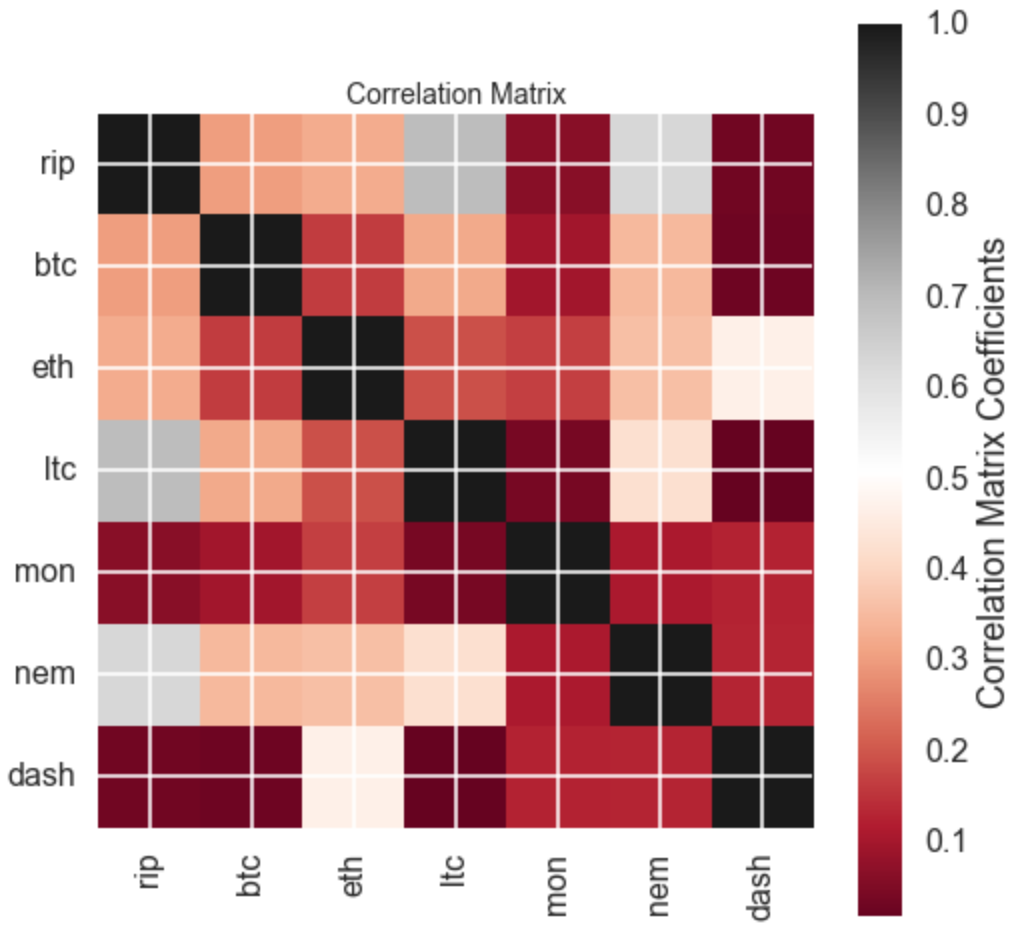
\includegraphics[scale=.7]{corr.png}
\bigbreak
\subsubsection*{Computing eigenvectors and corresponding eigenvalues}
\bigbreak
We will use Jacobi method to find eigenvalues and eigenvectors of correlation matrix since this method is a fairly robust way to extract all of the eigenvalues and eigenvectors of a symmetric matrix. The method is based on a series of rotations, called Jacobi or Givens rotations, which are chosen to eliminate off-diagonal elements while preserving the eigenvalues. Details of Jacobi method will be covered in Section xxx.
\bigbreak
We can check if the eigenvector-eigenvalue calculation is correct by using the equation:

$$M_{cov} u_i = \lambda_i u_i$$ where
\newline$M_{cov}$ = covariance matrix, 
\newline$u_i$ = the ith colummn of eigenvector matrix, 
\newline$\lambda_i$ = eigenvalue associated with $u_i$

\bigbreak
\subsubsection*{Sorting Eigenpairs \& Explained Variance}
\bigbreak
In order to decide which eigenvector(s) can dropped without losing too much information for the construction of lower-dimensional subspace, we need to inspect the corresponding eigenvalues: The eigenvectors with the lowest eigenvalues bear the least information about the distribution of the data; those are the ones can be dropped. In order to do so, the common approach is to rank the eigenvalues from highest to lowest in order choose the top k eigenvectors. The first principal component is required to have the largest possible variance.The second component is computed under the constraint of being orthogonal to the first component and to have the largest possible inertia. The other components are computed likewise.
\bigbreak
\begin{tabular}{ccc}
\hline
\head{Principal Component} & \head{Eigenvalue} & \head{Eigenvector}\\
\hline
1  & 2.654 & array([ 0.517,  0.334,  0.358,  0.455,  0.137,  0.487,  0.174])\\
2 & 1.376 &  array([ 0.237,  0.15 , -0.508,  0.309, -0.327,  0.063, -0.676])\\
3 & 0.941 & array([-0.105,  0.305, -0.204, -0.065,  0.88 , -0.037, -0.274])\\
4 & 0.769 & array([-0.286,  0.867,  0.007, -0.226, -0.311, -0.044,  0.13 ])\\
5 & 0.564 & array([-0.015, -0.095,  0.228, -0.611, -0.056,  0.64 , -0.39 ])\\
6 & 0.464 & array([-0.013, -0.064, -0.712, -0.087,  0.027,  0.472,  0.508])\\
7 & 0.239 & array([ 0.764,  0.091, -0.118, -0.511,  0.012, -0.351,  0.103])\\
\hline
\end{tabular}
$$\textbf{Table 1:  Eigenvalue and Eigenvector for each principal component}$$
\bigbreak
After sorting the eigenpairs, the next question is “how many principal components are we going to choose for our new feature subspace?” A useful measure is the proportion of variance, which can be calculated from the eigenvalues. The explained variance tells us how much information (variance) can be attributed to each of the principal components.
\bigbreak
Table 2 displays the results of a principal-component analysis of the cryptocurrencies’ daily returns: The eigenvalues, proportio of variance, and cumulative variance for each component. The single-strongest factor only explains 37.9$\%$ of the variation of crypto-currency returns. Moreover, each subsequent factor is providing only slowly declining additional information content, so that at least 5 factors are needed in order to account for 90$\%$ of the variation from these 7 crypto-currencies. 
\bigbreak
\begin{tabular}{cccc}
\hline
\head{Principal Component} & \head{Eigenvalue} & \head{Proportion of Variance} & \head{Cumulative Variance}\\
\hline
1 & 2.654 &  37.915\% & 37.915\%\\
2 & 1.376 & 19.635\% & 57.55\%\\
3 & 0.941 &  13.422\% & 70.972\%\\
4 & 0.769 &  10.967\% & 81.939\%\\
5 & 0.564 &  8.040\%  & 89.979\%\\
6 & 0.464 & 6.613\% & 96.592\%\\
7 & 0.239 &  3.408\% & 100\%\\
\hline
\end{tabular}
$$\textbf{Table 2:  Explained variance and cumulative varaince for each principal component}$$
\bigbreak
\textbf{??????
ADD (Comparison with XLE)}
\bigbreak

\subsubsection*{Component Loadings}
\bigbreak
In multivariate space, the correlation between the principal component and the original variables (crytocurrencies) is called the component loadings. Based on loadings, we can tell how much of the variation in a variable is explained by the component.
\bigbreak
Loadings = Orthonormal Eigenvectors $* \sqrt{Absolute Eigen values}$
\bigbreak
Principal component loading diagram is shown below:
\bigbreak
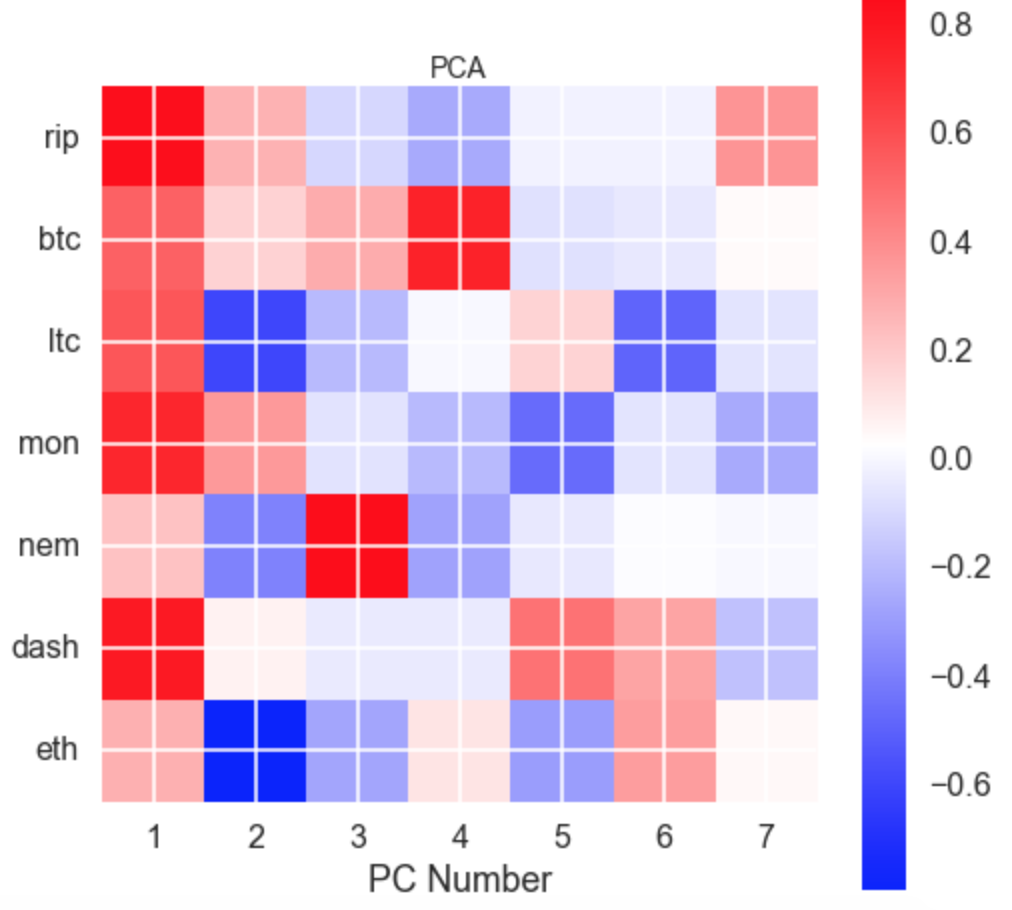
\includegraphics[scale=.6]{pca_loadings.png}
\bigbreak
\begin{tabular}{cccccccc}
\hline
\head{Principal \newline Component} & \head{Ripple} & \head{Bitcoin} & \head{Litecoin} &\head{Monero} &\head{Nem} &\head{Dash} &\head{Ethereum}\\
\hline
1 & 0.843&0.544&0.583&0.741&0.224&0.793&0.284\\
2 & 0.277&0.176&-0.595&0.363&-0.383&0.074	&-0.793\\
3 & -0.102	&0.295&-0.198&-0.063&0.853&-0.036&-0.266\\
4 & -0.250&0.760&0.006&-0.198&-0.272&-0.039&0.114\\
5 & -0.011	&-0.071&0.171&-0.459&-0.042&0.480&-0.293\\
6 & -0.009&-0.043&-0.484&-0.059&0.018&0.321&0.345\\
7 & 0.373&0.044&-0.058&-0.249&0.006&-0.171&0.050\\
\hline
\end{tabular}
$$\textbf{Table 3: Component Loadings}$$

\bigbreak
The first principal component is strongly correlated (loading score $\geq$ 0.7) with three out of seven currencies. The first principal component increases with increasing Ripple, Monero, and Dash scores. This suggests that these three currencies are likely to vary together (positvely correlated). If one increases, then the remaining ones tend to as well. Furthermore, we see that the correlation of first principal component with those six currencies are quite similar. \newline
We also notice that the second principal component (negatively) correlates most strongly with Ethereum. In fact, we could state that based on the correlations of -0.793, this principal component is primarily a measure of Ethereum.
\bigbreak
We construct the bi-plot of relative weights of each cryptocurrency in the first two PC components (PC-1 and PC-1) arising from the previous analysis:
\bigbreak
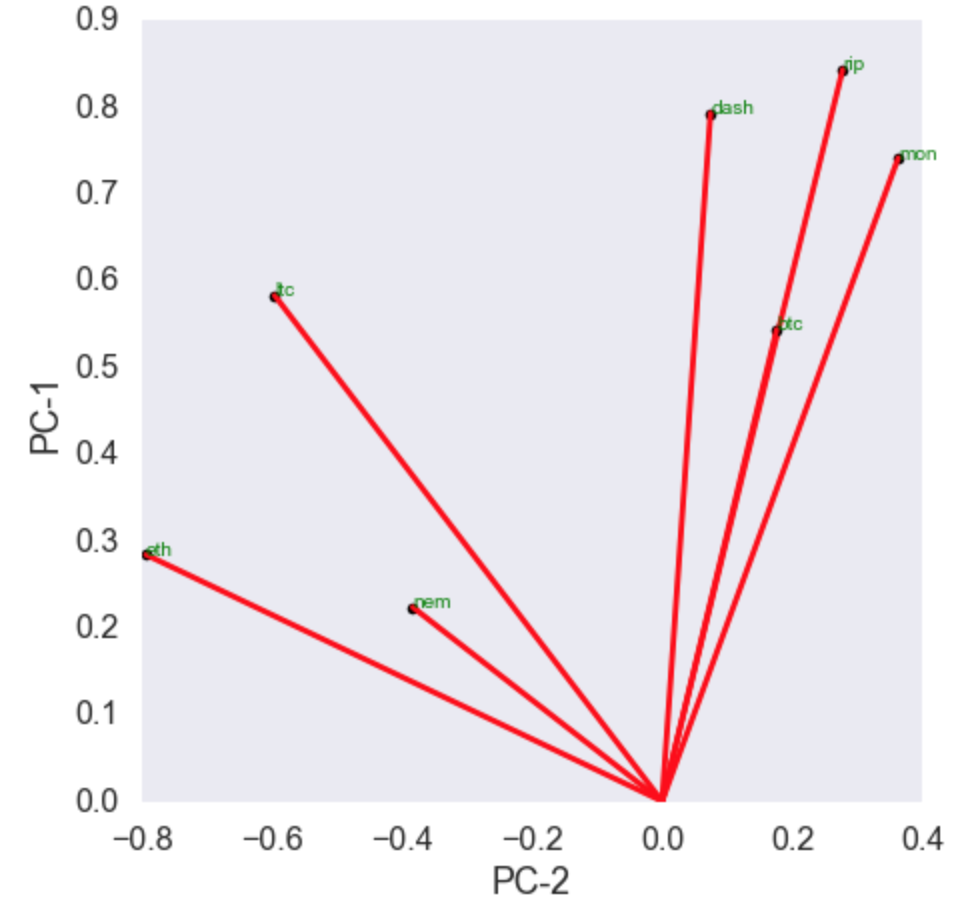
\includegraphics[scale=.6]{biplot1.png}
\bigbreak
This diagram also demonstrate the distinct movement between Ethereum and the rest of cryptocurrencies. All seven variables have positive values in the PC1 axis, while Litecoin, Nem, Ethereumare negative in PC2's and Ripple, Bitcoin, Monero and Dash is positive. Since all the variables are positive in PC1, those which constrain the system the most are Ripple and (then) Dash and Monero (in PC1 axis).The PC2, which has much smaller variance, contrasts Ethereum from everything else.
\bigbreak
The cosine of the angles between vectors is equal to the correlation between those variables. Hence vectors pointing in the same direction are perfectly correlated, and those at right angles are uncorrelated. As we can see, Ripple and Bitcoin are high correlation, while Ethereum has extreme low correlation with Bitcoin, Monero, and Ripple. This conclusion is also supported by the correlation matrix.

\bigbreak
In order to further confirm the weak correlation for each pair of currencies (cryptocurrency time-series), we make use of two distinct tools, namely, one-factor linear regression (hence its $R^2$ metric) and Kendall’s rank correlation metric of $\tau$. (NOT SURE IF WE NEED THIS.. DEPEND ON ANY SPACE LEFT)
\section*{3 - XXX}
\subsection*{(a) Introduction}
\end{document}







